% Organizing document for the HMMER User's Guide
%

\documentclass[11pt]{report}
\usepackage{fullpage}
\usepackage{times}
\usepackage{epsfig}
\usepackage{html}		% From the LaTeX2html translator
\usepackage{apalike}
\setcounter{secnumdepth}{1}

% customizations used in the User's Guide

\newenvironment{wideitem}{\begin{list} 
     {}
     { \setlength{\labelwidth}{2in}\setlength{\leftmargin}{1.5in}}}
     {\end{list}}

\newenvironment{miditem}{\begin{list} 
     {}
     { \setlength{\labelwidth}{1.5in}\setlength{\leftmargin}{1in}}}
     {\end{list}}

% need temp vars for parindent, parskip saving
%
\newlength{\sresavei}
\newlength{\sresaves}

% Consistent font styles
%   \prog{}  for a program or file name
%   \emprog{} for an emphasized program or file name
%   \user{}     for a typed used command
%   \begin{machine}  for machine output

\newcommand{\prog}[1]{\texttt{#1}}
\newcommand{\emprog}[1]{{\bfseries\texttt{#1}}}
\newcommand{\user}[1]{\noindent{\small\bfseries\texttt{$>$ #1}}\\}

\begin{document}
\bibliographystyle{apalike}

\begin{titlepage}
{\Large

\vspace*{\fill}

\begin{latexonly}
\noindent
{\Huge \textsf{HMMER User's Guide}} \\ 
\rule[2pt]{\textwidth}{1pt} \\
\hspace*{\fill} {\large \textsf{Biological sequence analysis using
profile hidden Markov models} \\ }
\end{latexonly}

\begin{htmlonly}
\begin{center}
{\Huge \textbf{HMMER User's Guide}}\\
{\large \textbf{Biological sequence analysis using
profile hidden Markov models}}\\
\end{center}
\end{htmlonly}

\vspace*{\fill}

\begin{center}
\textsl{\htmladdnormallink{http://hmmer.wustl.edu/}{http://hmmer.wustl.edu/}}\\
Version 2.1.1; December 1998 \\ 

\vspace*{\fill}

Sean Eddy\\
Dept. of Genetics, Washington University School of Medicine\\
4566 Scott Ave., St. Louis, MO 63110, USA\\
\textsl{eddy@genetics.wustl.edu} \\
With contributions by Ewan Birney (\textsl{birney@sanger.ac.uk})\\
\end{center}

\vspace*{\fill}

}
\end{titlepage}


\vspace*{\fill}
\begin{flushleft}
Copyright (C) 1992-1998, Washington University in St. Louis.\vspace{5mm}

Permission is granted to make and distribute verbatim copies of this
manual provided the copyright notice and this permission notice are
retained on all copies.\vspace{5mm}

The HMMER software package is a copyrighted work that may be freely
distributed and modified under the terms of the GNU General Public
License as published by the Free Software Foundation; either version 2
of the License, or (at your option) any later version. Some versions
of HMMER may have been obtained under specialized commercial licenses
from Washington University; for details, see the files COPYING and
LICENSE that came with your copy of the HMMER software.\vspace{5mm}

This program is distributed in the hope that it will be useful, but
WITHOUT ANY WARRANTY; without even the implied warranty of
MERCHANTABILITY or FITNESS FOR A PARTICULAR PURPOSE.\vspace{5mm}

See the Appendix for a copy of the full text of the GNU General Public
License.\vspace{5mm}

\end{flushleft}

\tableofcontents

\chapter{Tutorial}

I hate reading documentation. I just want examples of how stuff works,
just enough to get me started and doing something productive. So,
here's a tutorial walk-through of some small projects with HMMER. If
you want the introduction, that's the second chapter. The tutorial
should be sufficient to get you started on work of your own. You can
read the other chapters later if you want.

\section {The programs in HMMER}

There are currently nine programs supported in the HMMER 2 package:

\begin{wideitem}
\item[\emprog{hmmalign}] Align sequences to an existing model.
\item[\emprog{hmmbuild}] Build a model from a multiple sequence alignment.
\item[\emprog{hmmcalibrate}] Takes an HMM and empirically determines
parameters that are used to make searches more sensitive, by
calculating more accurate expectation value scores (E-values).
\item[\emprog{hmmconvert}] Convert a model file into different formats,
including a compact HMMER 2 binary format, and ``best effort''
emulation of GCG profiles.
\item[\emprog{hmmemit}] Emit sequences probabilistically from a profile HMM.
\item[\emprog{hmmfetch}] Get a single model from an HMM database.
\item[\emprog{hmmindex}] Index an HMM database.
\item[\emprog{hmmpfam}] Search an HMM database for matches to a query sequence.
\item[\emprog{hmmsearch}] Search a sequence database for matches to an HMM.
\end{wideitem}

HMMER also provides a number of utility programs which are not HMM
programs, but may be useful:

\begin{wideitem}
\item[\emprog{alistat}] Show some simple statistics about a sequence
alignment file.
\item[\emprog{getseq}] Retrieve a (sub-)sequence from a sequence file.
\item[\emprog{seqstat}] Show some simple statistics about a sequence file.
\item[\emprog{sreformat}] Reformat a sequence file into a different format.
\end{wideitem}

The following four programs are not included in the current release,
but are planned (i.e. they're vaporware, but it may be useful to you
to know that they're on the drawing board:)

\begin{wideitem}
\item[\emprog{hmmconfig}] Alter the search configuration of an existing model.
\item[\emprog{hmminfo}] Display summary information about the model(s) in a file.
\item[\emprog{hmmtrain}] Train a model from initially unaligned sequences,
producing both a model and a multiple alignment.
\item[\emprog{hmmview}] Graphical viewer and editor for HMMs.
\end{wideitem}

\section{Files used in the tutorial}

The subdirectory \prog{/Demos} in the HMMER distribution contains the
files used in the tutorial, as well as a number of examples of various
file formats that HMMER reads. The important files for the tutorial
are:

\begin{wideitem}
\item[\emprog{globins50.msf}] An MSF format alignment file of 50 aligned globin sequences.
\item[\emprog{ globins630.fa}] A FASTA format file of 630 unaligned globin sequences.
\item[\emprog{ fn3.slx}] A SELEX format alignment file of fibronectin type III domains.
\item[\emprog{ rrm.slx}] A SELEX format alignment file of RNA recognition
motif domains.
\item[\emprog{ pkinase.slx}] A SELEX format alignment file of protein kinase
catalytic domains.
\item[\emprog{ Artemia.fa}] A FASTA file of brine shrimp globin, which contains
nine tandemly repeated globin domains.
\item[\emprog{ 7LES\_DROME}] A SWISSPROT file of the {\em Drosophila} 
Sevenless sequence, a receptor tyrosine kinase with multiple domains.
\end{wideitem}

Create a new directory that you can work in, and copy all the files in
\prog{Demos} there. I'll assume for the following examples that you've
installed the HMMER programs in your path; if not, you'll need to give
a complete path name to the HMMER programs (e.g. something like \prog{
/usr/people/eddy/ hmmer-2.0/hmmbuild} instead of just \prog{hmmbuild}).

\section{Searching a sequence database with a single profile HMM}

One common use of HMMER is to search a sequence database for
homologues of a protein family of interest. You need a multiple
sequence alignment of the sequence family you're interested in.
(Profile HMMs can be trained from unaligned sequences; however, this
functionality is temporarily withdrawn from HMMER. I recommend
CLUSTALW as an excellent, freely available multiple sequence alignment
program.)

\subsection{HMM construction with \prog{ hmmbuild}}

Let's assume you have a multiple sequence alignment of a protein
domain or protein sequence family. To use HMMER to search for
additional remote homologues of the family, you want to first build a
profile HMM from the alignment. The following command builds a profile
HMM from the alignment of 50 globin sequences in \prog{ globins50.msf}:

\vspace{1.5em}
\user{hmmbuild globin.hmm globins50.msf}
\vspace{-1.5em}
{\small\begin{verbatim}
hmmbuild - build a hidden Markov model from an alignment
HMMER 2.0 (June 1998)
Copyright (C) 1992-1998 Washington University School of Medicine
HMMER is freely distributed under the GNU General Public License (GPL).
- - - - - - - - - - - - - - - - - - - - - - - - - - - - - - - - - - - -
Training alignment:                globins50.msf
Number of sequences:               50
Search algorithm configuration:    Multiple domain (hmmls)
Model construction strategy:       MAP (gapmax hint: 0.50)
Prior used:                        (default)
Prior strategy:                    Dirichlet
Sequence weighting method:         G/S/C tree weights
- - - - - - - - - - - - - - - - - - - - - - - - - - - - - - - -
Determining effective sequence number    ... done. [13]
Weighting sequences heuristically        ... done.
Constructing model architecture          ... done.
Converting counts to probabilities       ... done.
Setting model name, etc.                 ... done. [globins50]

Constructed a profile HMM (length 162)
Average score:      283.03 bits
Minimum score:      137.32 bits
Maximum score:      343.50 bits
Std. deviation:      53.21 bits

Finalizing model configuration           ... done.
Saving model to file                     ... done. [globin.hmm]
\end{verbatim}}

The process takes a second or two.  \prog{ hmmbuild} create a new HMM
file called \prog{ globin.hmm}. This is a human and computer readable
ASCII text file, but for now you don't care. You also don't care for
now what all the stuff in the output means; I'll describe it in detail
later. The profile HMM can be treated as a compiled model of your
alignment.

\subsection{HMM calibration with \prog{ hmmcalibrate}}

This step is optional, but doing it will increase the sensitivity of
your database search.

When you search a sequence database, it is useful to get ``E-values''
(expectation values) in addition to raw scores. When you see a
database hit that scores $x$, an E-value tells you the number of hits
you would've expected to score $x$ or more just by chance in a
sequence database of this size. 

HMMER will always estimate an E-value for your hits. However, unless
you ``calibrate'' your model before a database search, HMMER uses an
analytic upper bound calculation that is extremely conservative.  An
empirical HMM calibration costs time (about 10\% the time of a
SWISSPROT search) but it only has to be done once per model, and can
greatly increase the sensitivity of a database search. To empirically
calibrate the E-value calculations for the globin model, type:

\vspace{1.5em}
\user{hmmcalibrate globin.hmm}
\vspace{-1.5em}
{\small\begin{verbatim}
hmmcalibrate -- calibrate HMM search statistics
HMMER 2.0 (June 1998)
Copyright (C) 1992-1998 Washington University School of Medicine
HMMER is freely distributed under the GNU General Public License (GPL).
- - - - - - - - - - - - - - - - - - - - - - - - - - - - - - - - - - - -
HMM file:                 globin.hmm
Length distribution mean: 325
Length distribution s.d.: 200
Number of samples:        5000
random seed:              895790561
histogram(s) saved to:    [not saved]
- - - - - - - - - - - - - - - - - - - - - - - - - - - - - - - -

HMM    : globins50
mu     :  -107.928612
lambda :     0.186579
max    :   -63.859001
//
\end{verbatim}}

This takes several minutes. Go have a cup of coffee. When it is
complete, the relevant parameters are added to the HMM file.

Calibrated HMMER E-values tend to be relatively accurate. E-values of
0.1 or less are, in general, very significant hits. Uncalibrated HMMER
E-values are also reliable, erring on the cautious side; uncalibrated
models may miss remote homologues.

\subsection{Sequence database search with \prog{ hmmsearch}}

As an example of searching for new homologues using a profile HMM,
we'll use the globin model to search for globin domains in the example
{\em Artemia} globin sequence in \prog{ Artemia.fa}:

\vspace{1.5em}
\user{hmmsearch globin.hmm Artemia.fa}

The output comes in several sections, and unlike building and
calibrating the HMM (where we treated the HMM as a black box), now you
{\em do} care about what it's saying.

The first section is the {\em header} that tells you waht program you
ran, on what, and with what options:

{\small\begin{verbatim}
hmmsearch - search a sequence database with a profile HMM
HMMER 2.0 (June 1998)
Copyright (C) 1992-1998 Washington University School of Medicine
HMMER is freely distributed under the GNU General Public License (GPL).
- - - - - - - - - - - - - - - - - - - - - - - - - - - - - - - - - - - -
HMM file:                 globin.hmm [globins50]
Sequence database:        Artemia.fa
- - - - - - - - - - - - - - - - - - - - - - - - - - - - - - - -

Query HMM:  globins50  
  [HMM has been calibrated; E-values are empirical estimates]
\end{verbatim}}

The second section is the {\em sequence top hits} list. It is a list
of ranked top hits (sorted by E-value, most significant hit first),
formatted in a BLAST-like style:

{\small\begin{verbatim}
Scores for complete sequences (score includes all domains):
Sequence Description                                    Score    E-value  N 
-------- -----------                                    -----    ------- ---
S13421   S13421 GLOBIN - BRINE SHRIMP                   335.5     1e-101   8
\end{verbatim}}

The first field is the name of the target sequence, then followed by
the description line for the sequence. The last three fields are the
raw score (in units of ``bits''), the estimated E-value, and the total
number of domains detected in the sequence.  By default, every
sequence with an E-value over 10.0 is listed in this output.

The second section is the {\em domain top hits} list. By default, for
every sequence with an E-value less than 10, every domain with a
non-zero raw score is listed. (Read that carefully. In a later chapter
we'll discuss some caveats about how \prog{ hmmsearch} identifies
domains, and how to control its output in different ways.) Each domain
detected in the search is output in a list ranked by E-value:

{\small\begin{verbatim}
Parsed for domains:
Sequence Domain  seq-f seq-t    hmm-f hmm-t      score  E-value
-------- ------- ----- -----    ----- -----      -----  -------
S13421     6/8     928  1075 ..     1   162 []    65.8  1.5e-20
S13421     2/8     149   288 ..     1   162 []    59.4  1.3e-18
S13421     3/8     303   450 ..     1   162 []    58.4  2.6e-18
S13421     8/8    1238  1390 ..     1   162 []    42.5  1.6e-13
S13421     5/8     771   918 ..     1   162 []    33.8  3.3e-12
S13421     7/8    1085  1234 ..     1   162 []    32.0  4.6e-12
S13421     4/8     454   607 ..     1   162 []    26.1  1.4e-11
S13421     1/8       1   139 [.     1   162 []    21.9    3e-11
\end{verbatim}}

The first field is the name of the target sequence. The second field
is the number of this domain: e.g. ``6/8'' means the sixth domain of
eight total domains detected. 

The fields marked ``seq-f'' and ``seq-t'' mean ``sequence from'' and
``sequence to'': the start and end points of the alignment on the
target sequence. After these two fields is a shorthand annotation for
whether the alignment is ``global'' with respect to the sequence or
not. A dot (.) means the alignment does not go all the way to the end;
a bracket ([ or ]) means it does. Thus, .. means that the alignment is
local within the sequence; [. means that the alignment starts at the
beginning of the sequence, but doesn't go all the way to its end; .]
means the alignment starts somewhere internally and goes all the way
to the end; and [] means the alignment includes the entire sequence.

Analogously, the fields marked ``hmm-f'' and ``hmm-t'' indicate the
start and end points with respect to the consensus coordinates of the
model, and the following field is a shorthand for whether the
alignment is global with respect to the {\em model}. Here, for
instance, all the globin domains in the {\em Artemia} sequence are
complete matches to the entire globin model -- {\em because, by
default, \prog{ hmmbuild} built the HMM to only look for those kinds of
alignments}. We'll discuss later how to modify the profile HMM for
other search styles.

The final two fields are the raw score in bits and the estimated
E-value, {\em for the isolated domain}. Because of the method HMMER
uses to correct raw scores for biased sequence composition, the raw
scores for the domains do not necessarily sum up to the raw score of
the sequence.

The next section is the {\em alignment output}. By default, every
domain that appeared in the domain top hits list now appears as a
BLAST-like alignment. For example:

{\small\begin{verbatim}
Alignments of top-scoring domains:
S13421: domain 6 of 8, from 928 to 1075: score 65.8, E = 1.5e-20
                   *->vilealvnssShLSaeekalVkslWYgKVegnaeeiGaeaLgRlFvv
                      +           LSa e a Vk++W   V+ ++ ++G  ++  lF +
      S13421   928    G-----------LSAREVAVVKQTW-NLVKPDLMGVGMRIFKSLFEA 962  

                   YPwTqryFphFgdLssldavkgspkvKaHGkKVltalgdavkhLDdtgnl
                   +P  q+ Fp+F+d+ +ld +++ p v +H   V t l++ ++ LD   nl
      S13421   963 FPAYQAVFPKFSDV-PLDKLEDTPAVGKHSISVTTKLDELIQTLDEPANL 1011 

                   kgalakLSelHadklrVDPeNFklLghvlvvvLaehfgkdftPevqAAwd
                   +    +L+e H   lrV+   Fk +g+vlv  L   +g  f+  +  +w 
      S13421  1012 ALLARQLGEDH-IVLRVNKPMFKSFGKVLVRLLENDLGQRFSSFASRSWH 1060 

                   KflagvanaLahKYr<-*
                   K++++++  +++      
      S13421  1061 KAYDVIVEYIEEGLQ    1075 
\end{verbatim}}

The top line is the HMM consensus. The amino acid shown for the
consensus is the highest probability amino acid at that position
according to the HMM (not necessarily the highest {\em scoring} amino
acid, though). Capital letters mean ``highly conserved'' residues:
those with a probability of $> 0.5$ for protein models, or $> 0.9$ for
DNA models. 

The center line shows letters for ``exact'' matches to the highest
probability residue in the HMM, or a ``+'' when the match has a
positive score and is therefore considered to be ``conservative''
according to the HMM's view of {\em this particular position in the
model} -- not the usual definition of conservative changes in general.

The third line shows the sequence itself, of course.

The next section of the output is the {\em score histogram}.  It shows
a histogram with raw score increasing along the Y axis, and the number
of sequence hits represented as a bar along the X axis. In our example
here, since there's only a single sequence, the histogram is very
boring:

{\small\begin{verbatim}
Histogram of all scores:
score    obs    exp  (one = represents 1 sequences)
-----    ---    ---
  335      1      0|=                                                          
\end{verbatim}}

Notice though that it's a histogram of the whole sequence hits, not
the domain hits.

You can ignore the rest of the \prog{ hmmsearch} output:

{\small\begin{verbatim}
% Statistical details of theoretical EVD fit:
              mu =  -107.9286
          lambda =     0.1866
chi-sq statistic =     0.0000
  P(chi-square)  =          0

Whole sequence top hits:
tophits_s report:
     Total hits:           1
     Satisfying E cutoff:  1
     Total memory:         15K

Domain top hits:
tophits_s report:
     Total hits:           8
     Satisfying E cutoff:  8
     Total memory:         20K
\end{verbatim}}

This is just some trailing internal info about the search that's
useful to me sometimes, but probably not to you.

\subsection{Searching major databases like NR or SWISSPROT}

HMMER reads all major database formats and does not need any special
database indexing. You can search any large sequence database you have
installed locally just by giving the full path to the database file,
e.g. something like:

\vspace{1.5em}
\user{hmmsearch globin.hmm /nfs/databases/swiss35/sprot35.dat}

If you have BLAST installed locally, it's likely that you have a
directory (or directories) in which the BLAST databases are kept.
These directories are specified in an environment variable called \prog{
BLASTDB}. HMMER will read the same environment variable. For example,
if you have a BLAST database called \prog{
/nfs/databases/blast-db/swiss35}, the following commands will work:

\vspace{1.5em}
\user{setenv BLASTDB /nfs/databases/blast-db/}
\user{hmmsearch globin.hmm swiss35}

Obviously, you'd tend to have the \prog{ setenv} command as part of the
local configuration of your machine, rather than typing it at the
command line.

\subsection{Local alignment searches with \prog{ hmmsearch}}

{\em This is extremely important.} HMMER does not do local
(Smith/Waterman) and global (Needleman/Wunsch) style alignments in the
same way that most computational biology analysis programs do it.  To
HMMER, whether local or global alignments are allowed is part of the
{\em model}, rather than being accomplished by running a different
{\em algorithm}. (This will be discussed in greater detail later; it
is part of the ``Plan7'' architecture of the new HMMER2 models.)

Therefore, you need to choose what kind of alignments you want to
allow {\em when you build the model} with \prog{ hmmbuild}.  By default,
\prog{ hmmbuild} builds models which allow alignments that are global
with respect to the HMM, local with respect to the sequence, and
allows multiple domains to hit per sequence. Such models will only
find complete domains. 

\prog{ hmmbuild} provides some standard options for common alignment
styles. The following table shows the four alignment styles supported
by \prog{ hmmbuild}, and also shows the equivalent old HMMER 1.x search
program style (to orient experienced HMMER users).

\vspace{1em}
\begin{tabular}{lllll}
Command           & w.r.t. sequence & w.r.t. HMM & multidomain & HMMER
1 equivalent \\ \hline
\prog{ hmmbuild}    & local & global & yes & hmmls \\
\prog{ hmmbuild -f} & local & local  & yes & hmmfs \\
\prog{ hmmbuild -g} & local & global & no  & hmms  \\
\prog{ hmmbuild -s} & local & local  & no  & hmmsw \\ \hline
\end{tabular}
\vspace{1em}

In brief, if you want maximum sensitivity at the expense of only
finding complete domains, use the \prog{ hmmbuild} default. If you need
to find fragments (local alignments) too, and are willing to give up
some sensitivity to see them, use \prog{ hmmbuild -f}. If you want the
best of both worlds, build two models and search with both of them.

\section{Searching a query sequence against a profile HMM database}

A second use of HMMER is to look for known domains in a query
sequence, by searching a single sequence against a library of
HMMs. (Contrast the previous section, in which we searched a single
HMM against a sequence database.) To do this, you need a library of
profile HMMs. One such library is our PFAM database
\cite{Sonnhammer97,Sonnhammer98}, and you can also create your own.

\subsection{Creating your own profile HMM database} 

HMM databases are simply concatenated single HMM files. You can build
them either by invoking the \prog{ -A} ``append'' option of \prog{
hmmbuild}, or by concatenating HMM files you've already built.  For
example, here's two ways to build an HMM database called \prog{ myhmms}
that contains models of the rrm RNA recognition motif domain, the fn3
fibronectin type III domain, and the pkinase protein kinase catalytic
domain:

\vspace{1.5em}
\user{hmmbuild rrm.hmm rrm.slx}
\user{hmmbuild fn3.hmm fn3.slx}
\user{hmmbuild pkinase.hmm pkinase.slx}
\user{cat rrm.hmm fn3.hmm pkinase.hmm > myhmms}
\user{hmmcalibrate myhmms}

or:

\vspace{1.5em}
\user{hmmbuild -A myhmms rrm.slx }
\user{hmmbuild -A myhmms fn3.slx }
\user{hmmbuild -A myhmms pkinase.slx }
\user{hmmcalibrate myhmms }

Notice that \prog{ hmmcalibrate} can be run on HMM databases as well as
single HMMs.

\subsection{Parsing the domain structure of a sequence with \prog{ hmmpfam}}

Now that you have a small HMM database called \prog{ myhmms}, let's use
it to analyze the {\em Drosophila} Sevenless sequence, \prog{
7LES\_DROME}:

\vspace{1.5em}
\user{hmmpfam myhmms 7LES\_DROME }

Like \prog{ hmmsearch}, the \prog{ hmmpfam} output comes in several
sections. The first section is the {\em header}:

{\small\begin{verbatim}
hmmpfam - search a single seq against HMM database
HMMER 2.0 (June 1998)
Copyright (C) 1992-1998 Washington University School of Medicine
HMMER is freely distributed under the GNU General Public License (GPL).
- - - - - - - - - - - - - - - - - - - - - - - - - - - - - - - - - - - -
HMM file:                 myhmms
Sequence file:            7LES_DROME
- - - - - - - - - - - - - - - - - - - - - - - - - - - - - - - -
Query:  7LES_DROME  SEVENLESS PROTEIN (EC 2.7.1.112).
\end{verbatim}}

The next section is the {\em sequence family classification} top hits
list, ranked by E-value. The scores and E-values here reflect the
confidence that this query sequence contains one {\em or more} domains
belonging to a domain family. The fields have the same meaning as in
\prog{ hmmsearch} output, except that the name and description are for
the HMM that's been hit.

{\small\begin{verbatim}
Scores for sequence family classification (score includes all domains):
Sequence Description                                    Score    E-value  N 
-------- -----------                                    -----    ------- ---
pkinase                                                 303.3      3e-87   1
fn3                                                     171.8    1.1e-47   6
\end{verbatim}}

The next section is the {\em domain parse} list, ordered by position
on the sequence (not by score). Again the fields have the same meaning
as in \prog{ hmmsearch} output:

{\small\begin{verbatim}
Parsed for domains:
Sequence Domain  seq-f seq-t    hmm-f hmm-t      score  E-value
-------- ------- ----- -----    ----- -----      -----  -------
fn3        1/6     437   522 ..     1    84 []    48.0  2.1e-10
fn3        2/6     825   914 ..     1    84 []    12.6     0.21
fn3        3/6    1292  1389 ..     1    84 []    15.2     0.13
fn3        4/6    1799  1891 ..     1    84 []    62.4  9.4e-15
fn3        5/6    1899  1978 ..     1    84 []    13.7     0.17
fn3        6/6    1993  2107 ..     1    84 []    18.4    0.067
pkinase    1/1    2209  2483 ..     1   278 []   303.3    3e-87
\end{verbatim}}

The final output section is the {\em alignment output}, just like \prog{
hmmsearch}:

{\small\begin{verbatim}
Alignments of top-scoring domains:
fn3: domain 1 of 6, from 437 to 522: score 48.0, E = 2.1e-10
                   *->P.saPtnltvtdvtstsltlsWsppt.gngpitgYevtyRqpkngge
                      P saP   + +++ ++ l ++W p +  ngpi+gY+++  ++++g+ 
  7LES_DROME   437    PiSAPVIEHLMGLDDSHLAVHWHPGRfTNGPIEGYRLRL-SSSEGNA 482  

                   wneltvpgtttsytltgLkPgteYtvrVqAvnggG.GpeS<-*
                   + e+ vp+   sy+++ L++gt+Yt+ +  +n +G+Gp     
  7LES_DROME   483 TSEQLVPAGRGSYIFSQLQAGTNYTLALSMINKQGeGPVA    522  
...
\end{verbatim}}

\subsection{Downloading the PFAM database}

The PFAM database is available from either \htmladdnormallink{\prog{
http://pfam.wustl.edu/}}{http://pfam.wustl.edu/} or \linebreak 
\htmladdnormallink{\prog{http://www.sanger.ac.uk/Pfam/}}{http://www.sanger.ac.uk/Pfam/}.
Download instructions are on the Web page. The PFAM HMM library is a
single large file, containing several hundred models of known protein
domains. Install it in a convenient directory and name it something
simple like \prog{ pfam}.

HMMER will look for PFAM and other files in a directory (or
directories) specified by the \prog{ HMMERDB} environment variable.  For
instance, if you install the PFAM HMM library as \linebreak \prog{
/nfs/databases/hmmer/pfam}, the following commands will search 
for domains in \prog{ 7LES\_DROME}:

\vspace{1.5em}
\user{setenv HMMERDB /nfs/databases/hmmer/}
\user{hmmpfam pfam 7LES\_DROME}

\section{Maintaining multiple alignments with \prog{ hmmalign}}

Another use of profile HMMs is to create multiple sequence alignments
of large numbers of sequences. A profile HMM can be build of a
``seed'' alignment of a small number of representative sequences, and
this profile HMM can be used to efficiently align any number of
additional sequences. 

This is in fact how the PFAM database is updated as the main SPTREMBL
database increases in size. The PFAM seed alignments are (relatively)
stable from release to release; PFAM full alignments are created
automatically by searching SPTREMBL with the seed model and aligning
all the significant hits into a multiple alignment using \prog{
hmmalign}.

For example, to align the 630 globin sequences in \prog{ globins630.fa}
to our globin model \prog{ globin.hmm}, and create a new alignment file
called \prog{ globins630.ali}, we'd do:

\vspace{1.5em}
\user{hmmalign -o globins630.ali globin.hmm globins630.fa}
\vspace{-1.5em}
{\small\begin{verbatim}
hmmalign - align sequences to an HMM profile
HMMER 2.0 (June 1998)
Copyright (C) 1992-1998 Washington University School of Medicine
HMMER is freely distributed under the GNU General Public License (GPL).
- - - - - - - - - - - - - - - - - - - - - - - - - - - - - - - - - - - -
HMM file:             globin.hmm
Sequence file:        globins630.fa
- - - - - - - - - - - - - - - - - - - - - - - - - - - - - - - -

Alignment saved in file globins630.ali
\end{verbatim}}

Using the \prog{ -o} option to specify a save file for the final
alignment is a good idea; else, the alignment will be displayed on the
screen as output (and an alignment of several hundred sequences will
give a fairly voluminous output).

\chapter{Introduction}

You discover a new protein sequence family, and carefully construct a
multiple sequence alignment. Your family, like most protein families,
has a number of strongly (but not absolutely) conserved key residues,
separated by characteristic spacing. You wonder if there are more
members of your family in the sequence databases, but the family is so
evolutionarily diverse, a BLAST search with any individual sequence
doesn't even find the rest of the sequences you already know about;
you're sure there are some distantly related sequences in the
``noise''. You spend many pleasant evenings scanning weak BLAST
alignments by eye to find ones with the right key residues are in the
right places. You sure wish there was a computer program that did this
better.

You get the sequence of another favorite protein and eagerly BLAST it
against the NCBI server, and nothing significant shows up. It looks
like you'll get no easy information from the sequence.

You BLAST another favorite sequence against the NCBI server; a
thousand hits come back, and the top hundred are hypothetical
sequences from genome projects. It looks like you'll have to wade
through a lot of BLAST output to find the informative hits.

Another sequence comes back a slew of hits to receptor tyrosine
kinases, but before you decide to call your sequence an RTK homologue,
you recall that RTK's are, like many proteins, composed of multiple
functional domains. Is your sequence really an RTK? Or is it a novel
sequence that also happens to have a protein kinase catalytic domain,
fibronectin type III domain, or immunoglobulin superfamily domain?

These (and other problems in sequence analysis) are the kinds of
problems that HMMER tries to address. 

\section {Profile HMMs}

Profile hidden Markov models (profile HMMs) are statistical models of
the primary structure consensus of a sequence family. Anders Krogh,
David Haussler, and co-workers at UC Santa Cruz introduced profile
HMMs \cite{Krogh94}, adopting HMM techniques which have been used for
years in speech recognition. HMMs had been used in biology before the
Krogh/Haussler work, but the Krogh paper had a particularly dramatic
impact, because HMM technology was so well-suited to the popular
``profile'' methods for searching databases using multiple sequence
alignments instead of single query sequences. Since then, several
computational biology groups (including ours) have rapidly adopted
HMMs as the underlying formalism for sequence profile analysis.

``Profiles'' were introduced by Gribskov and colleagues
\cite{Gribskov87,Gribskov90} at about the same time
that other groups introduced similar approaches, such as ``flexible
patterns'' \cite{Barton90}, and
``templates''\cite{Bashford87,Taylor86}. The term ``profile'' has
stuck.\footnote{There has been some agitation to call all such models
``position specific scoring matrices'', PSSMs, but certain small
nocturnal North American marsupials have a prior claim on the
mnemonic.}  All of these are more or less statistical descriptions of
the consensus of a multiple sequence alignment. They use
position-specific scores for amino acids (or nucleotides) and position
specific scores for opening and extending an insertion or deletion.
Traditional pairwise alignment (for example, BLAST
\cite{Altschul90}, FASTA \cite{Pearson88}, or the Smith/Waterman
algorithm \cite{Smith81}) uses position-{\em independent} scoring
parameters. This property of profiles captures important information
about the degree of conservation at various positions in the multiple
alignment, and the varying degree to which gaps and insertions are
permitted.

The advantage of using HMMs is that HMMs have a formal probabilistic
basis. We can use Bayesian probability theory to guide how all the
probability (scoring) parameters should be set. Though this might
sound like a purely academic issue, this probabilistic basis lets us
do things that the more heuristic methods cannot do easily. For
example, an HMM can be trained from unaligned sequences, if a trusted
alignment isn't yet known. Another consequence is that HMMs have a
consistent theory behind gap and insertion scores.\footnote{
Surprisingly, this is still controversial.  People have been saying
``there is no theory for setting gap scores'' for so long that many
people believe it.} In most details, HMMs are a slight improvement
over a carefully constructed profile -- but far less skill and manual
intervention is necessary to train a good HMM and use it.  This allows
us to make libraries of hundreds of profile HMMs and apply them on a
very large scale to whole-genome or EST sequence analysis.  One such
database of protein domain models is Pfam \cite{Sonnhammer97}; the
construction and use of Pfam is tightly tied to the HMMER software
package.

HMMs do have important limitations. One is that HMMs do not capture
any higher-order correlations.  An HMM assumes that the identity of a
particular position is independent of the identity of all other
positions.\footnote{This is not strictly true. There is a subtle
difference between an HMM's state path (a first order Markov chain)
and the sequence described by an HMM (generated from the state path by
independent emissions of symbols at each state).} HMMs make poor
models of RNAs, for instance, because an HMM cannot describe base
pairs. Also, compare protein ``threading'' methods, which include
scoring terms for nearby amino acids in a three-dimensional protein
structure. 

A general definition of HMMs and an excellent tutorial introduction to
their use has been written by Rabiner \cite{Rabiner89}. Throughout, I
will often use ``HMM'' to refer to the specific case of profile HMMs
as described by Krogh et al. \cite{Krogh94}. This shorthand usage is
for convenience only. For a review of profile HMMs, see \cite{Eddy96},
and for a complete book on the subject of probabilistic modeling in
computational biology, see \cite{Durbin98} 
\begin{htmlonly}
\htmladdnormallink{[More information on-line]}
{http://www.genetics.wustl.edu/eddy/publications/cupbook.html}
\end{htmlonly}.

\section{Primary changes from HMMER 1.x}

HMMER 2 is an almost complete rewrite of the original 1992-1996 HMMER
code. A list of the major changes follows.

\begin{wideitem}

\item [\textbf{Plan7}] The model architecture is changed. The ``Plan 7''
architecture\footnote{The origin of the codename is obscure, involving
both details of the state transition probability distributions in
profile HMM architecture and an inordinate fondness for bad science
fiction movies. Frighteningly, David Haussler understood the codename
immediately.} allows detailed control over parameters of local,
global, and multidomain alignments. In Plan 7, you choose the
alignment style when you build the model with \prog{hmmbuild}, not
when you search. A single database search program \prog{hmmsearch}
replaces the four search programs in HMMER 1.x.

\item [\textbf{Pfam support}] There is much better support for the Pfam
HMM database. HMMs have names; the HMM file format allows libraries of
multiple HMMs per file; and there is a search program
\prog{hmmpfam}
for searching a single query sequence against an HMM library.
HMM databases like Pfam can be indexed for rapid access using
\prog{hmmindex}, and single HMMs can be retrieved from an HMM
database using \prog{hmmfetch}.

\item [\textbf{E-values}] HMMER now reports both log-odds scores and
a E-value. E-values can detect significant matches even when the
log-odds score is negative. A new program \prog{hmmcalibrate}
empirically determines the necessary parameters for estimating
E-values as best as possible.

\item [\textbf{Output}] Database searches now sort and postprocess their results for
prettier and more useful output. Output styles are deliberately
similar to BLAST, to try to simplify the design of postprocessors.

\item [\textbf{Save file format}] HMMER save files are now in an ASCII format which
  is easy for humans to read, portable across all architectures
  without byteswapping issues, and compact.

\item [\textbf{Decent defaults}] The ``best'' average behavior of HMMER is now its
default behavior. For example, mixture Dirichlet priors are now the
default for protein model building. In HMMER 1.x, you had to invoke a
number of ``experimental'' options to get better performance -- this
led to a bunch of really frustrating benchmarking in the literature,
in which people compared fully optimized program X to the default
behavior of HMMER 1, which was the 1994 basic Krogh/Haussler behavior
rather than its actual power. (However, there's still a lot of bad
benchmarking, because people don't understand how to benchmark profile
software yet.)

\end{wideitem}

\section{Plan 7}

\subsection{The Plan 7 architecture}

The Plan 7 architecture is substantially different from the original
HMMER model architecture. 

The abbreviations for the states are as follows:

\begin{wideitem}
\item [\textbf{M$_x$}] Match state $x$.  Has $K$ emission probabilities.
\item [\textbf{D$_x$}] Delete state $x$. Non-emitter.
\item [\textbf{I$_x$}] Insert state $x$. Has $K$ emission probabilities.
\item [\textbf{S}]     Start state. Non-emitter.
\item [\textbf{N}]     N-terminal unaligned sequence state. 
    Emits \textit{on transition} with $K$ emission probabilities.
\item [\textbf{B}]     Begin state (for entering main model). Non-emitter.
\item [\textbf{E}]     End state (for exiting main model). Non-emitter.
\item [\textbf{C}]     C-terminal unaligned sequence state.
    Emits \textit{on transition} with $K$ emission probabilities.
\item [\textbf{J}]     Joining segment unaligned sequence state.
    Emits \textit{on transition} with $K$ emission probabilities.
\end{wideitem}

\begin{figure}
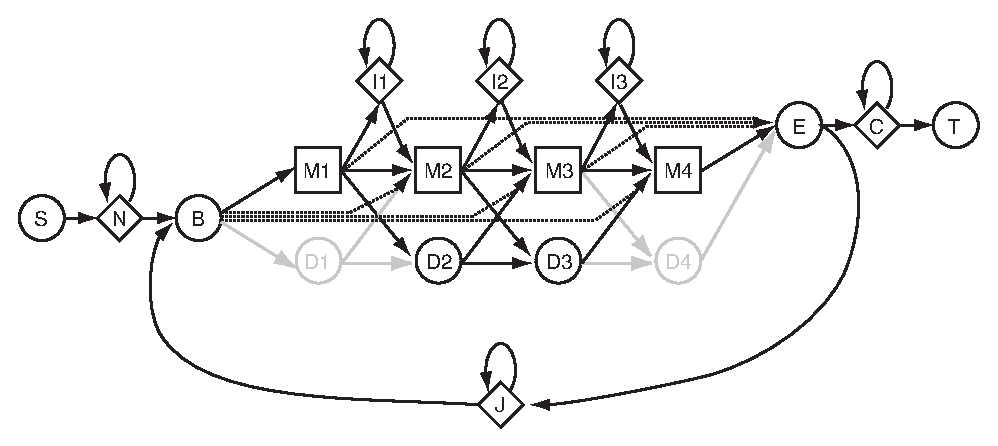
\epsfig{file=plan7.eps}
\caption{\textit{The Plan7 architecture. Squares indicate match states
(modeling consensus positions in the alignment). Diamonds indicate
insert states (modeling insertions relative to consensus) and special
random sequence emitting states. Circles indicate delete states
(modeling deletions relative to consensus) and special begin/end
states. Arrows indicate state transitions. See text for more details.}}
\end{figure}

The section of the model composed of M, D, and I states, and the B and
E states, is essentially a Krogh/Haussler profile HMM. I refer to this
as the ``main model''. A group of three states M/D/I at the same
consensus position in the alignment is called a ``node''. The main
model controls the \textit{data dependent} features of the model.  The
probability parameters in the main model are generally learned from
data in a multiple sequence/structure alignment.

Unlike the original Krogh/Haussler and HMMER model architecture, Plan
7 has no D $\rightarrow$ I or I $\rightarrow$ D transitions. This
reduction from 9 to 7 transitions per node in the main model is the
origin of the codename Plan 7. (The original HMMER architecture is
called Plan 9 in parts of the code.)

The other states (S,N,C,T,J) are called ``special states''. They
(combined with special entry probabilities from B and exit
probabilities to E) control the \textit{algorithm dependent} features
of the model: how likely the model is to generate various sorts of
local or multihit alignments. The algorithm dependent parameters are
typically not learned from data, but rather set externally by choosing
a desired alignment style.

\subsection{Local alignments in Plan 7}

The Plan 7 architecture models a complete sequence, regardless of how
much of that sequence matches the main model. \textit{All alignments
to a Plan 7 model are ``global'' alignments}, but some of the sequence
may be assigned to Plan 7 states (N,C,J) that generate ``random''
sequence that is not aligned to the main model.  Thus, the algorithm
dependent parts of the model control the \textit{apparent} locality of
the alignments.

Local alignments with respect to the sequence (i.e., allowing a match
to the main model anywhere internal to a longer sequence) are
controlled by the N and C states. If the N $\rightarrow$ N transition
is set to 0, alignments are constrained to start in the main model at
the very first residue. Similarly, if the C $\rightarrow$ C transition
is set to 0, alignments are constrained to match the main model at the
very last residue in the sequence.

Local alignments with respect to the model (i.e., allowing fragments
of the model to match the sequence) are controlled by B $\rightarrow$
M ``entry'' transitions and M $\rightarrow$ E ``exit'' transitions,
shown as dotted lines in the Plan 7 figure. Setting all entries but
the B $\rightarrow$ M$_1$ transition to 0 forces a partially
``global'' alignment in which all alignments to the main model must
start at the first match or delete state. Setting all exits to 0 but
the final M $\rightarrow$ E transition (which is always 1.0) forces a
partially global alignment in which all alignments to the main model
must end at the final match or delete state.

Multiple hit alignments are controlled by the E $\rightarrow$ J
transition and the J state. If the E $\rightarrow$ J transition is set
to 0, a sequence may only contain one domain (one alignment to the
main model). If it is nonzero, more than one domain per sequence can
be aligned to the main model. The J $\rightarrow$ J transition
controls the expected length of the intervening sequence between
domains; the lower this probability, the more clustered the domains
are expected to be.

The original HMMER1 search programs are encoded in Plan 7 models as
follows:

\begin{wideitem}
\item [\emprog{hmms}] Simple global alignment. $t_{NN}$ and $t_{CC}$ set to
$t_{GG}$ from the null model (see below). $t_{EJ}$ set to
zero. Internal entries and exits set to zero.

\item [\emprog{hmmls}] Akin to ``profile'' alignment (as Waterman and others
call it): global with respect to main model, local with respect to
sequence, multiple nonoverlapping domains allowed. $t_{NN}$ and
$t_{CC}$ set to $t_{GG}$ from the null model. $t_{EJ}$ set to
0.5. Internal entries and exits set to zero.
 
\item [\emprog{hmmsw}] Smith/Waterman alignment: fully local with 
respect to both the main model and the sequence; single domain.
$t_{NN}$ and $t_{CC}$ set to $t_{GG}$ from the null model. $t_{EJ}$
set to zero. Internal entries are set to $0.5/(M-1)$ for a model with
$M$ match states. Exit probabilities are set such that the overall
chance of exiting from an internal match state is 0.5, and the
posterior probability distribution over which match state is exited is
equal (I'm trying to word this carefully; the M $\rightarrow$ E
probabilities are not equal, because there's a small compensation for
the fact that if you can leave from $M_5$, then the chance that you'll
even get to $M_6$ is reduced.)

\item [\emprog{hmmfs}] Multihit Smith/Waterman alignment. Same
as the above, but $t_{EJ}$ is set to 0.5.
\end{wideitem}


One advantage of Plan 7 is great flexibility in choosing an alignment
style. Complicated alignment styles are easily encoded in the model
parameters without changing the alignment algorithm.  For example, say
you wanted to model human L1 retrotransposon elements. Because of the
way L1 elements are inserted by reverse transcriptase (RVT), L1
elements tend to have a defined 3' end (RVT starts replication at the
same place in each new L1) but a ragged 5' end (RVT prematurely falls
off a new L1 in an unpredictable fashion). A specialized L1 model
could define non-zero internal entry probabilities and zero internal
exit probabilities to model this biological situation.

One disadvantage of Plan 7 is that if you decide you want to do both
local and global alignments, you need two different models (or you
need to do one search, then change the model). This wouldn't be a
terrible burden except for the fact that the algorithm-dependent
parameters strongly affect the values of the $\mu$ and $\lambda$
parameters that E-value statistics depend on. If the algorithm
dependent parameters are changed, these parameters are lost and the
model should be recalibrated with \prog{hmmcalibrate} -- and
\prog{hmmcalibrate} is relatively slow.


\subsection{The Plan 7 null model}

When HMM alignments are scored, they are scored by a log-odds score
relative to a ``null model'' of random sequence composition
\cite{Barrett97}. In Plan 7, this model is now specified as a full
probabilistic model too:

\begin{center}
\epsfig{file=nullmodel.eps}
\end{center}

The G state has a symbol emission probability distribution for $K$
symbols in the alphabet. By default, this distribution is set either
to the average amino acid composition of SWISSPROT 34, or to 0.25 for
each nucleotide. The G $\rightarrow$ G transition controls the
expected length of observed random sequences; in practice, this
transition probability is so close to 1 that it has very little
effect. The F state is just a dummy end state like the T state in the
Plan 7 architecture.

\subsection{Wing retraction in Plan 7 dynamic programming}

In the figure of the Plan 7 architecture, you may have noticed that
the first and last delete states are greyed out. Internally in HMMER,
these delete states exist in the ``probability form'' of the model
(when the model is being worked with in every way except alignments)
but they are carefully removed in the ``search form'' of the model
(when the model is converted to log-odds scores and used for
alignments). This process is called ``wing retraction'' in the code,
by analogy to a swept-wing fighter changing from a wings-out takeoff
and landing configuration to a wings-back configuration for high speed
flight.

The problem is that the Plan 7 model allows cycles through the J
state. If a continuous nonemitting ``mute cycle'' were possible (J, B,
D states, E, and back to J), dynamic programming recursions would
fail. This is why special mute states like delete states must be
handled carefully in HMM dynamic programming algorithms; see
\cite{Durbin98} for further discussion. The easiest way to
prevent a mute cycle is to make sure that the model must pass through
at least one match state per path through the main model.

Wing retraction involves folding the probabilities of the terminal
delete paths into the Plan 7 entry and exit probabilities. For
example, in wing retraction the ``algorithm dependent'' B
$\rightarrow$ M$_{3}$ entry probability is incremented by the
probability of the ``data dependent'' path B $\rightarrow$ D$_1$
$\rightarrow$ D$_2$ $\rightarrow$ M$_3$.

Having the wing retraction step, rather than {\em always} folding
these probabilities together, is a design decision, preserving a
distinction between the ``algorithm dependent'' and ``data dependent''
parts of the model.

\section{Sequence file formats}

For all the programs, unaligned sequence files can be in FASTA,
Genbank, EMBL, or SWISS-PROT format, as well as a few other common
file formats. The programs automatically detect what format the file
is in and whether the sequences are DNA, RNA, or protein.

Aligned sequence files can be in ClustalW, GCG MSF, or SELEX
format. SELEX format is a simple format of one line per sequence,
containing the name first, followed by the aligned sequence. ClustalW,
MSF and SELEX alignment files can also be used where unaligned format
files are required; the sequences will be read in and their gaps
removed. 

Full specifications of these file formats and the other formats
recognized by the HMM package are in the file formats chapter near the
end of the guide.

The programs work on RNA, DNA, and protein sequence. They
automatically detect what your sequences are. The behavior of the
programs when a nucleic acid model is used to analyze protein
sequences, or vice versa, is undefined. Certain other situations may
arise (trying to search the ``complementary strand'' of a protein
database, for example) that are nonsensical in certain contexts. Be
forewarned. If you're lucky, the software will issue a snide warning
to you if you try to do something nonsensical, but usually it will
assume you know what you're doing.

\section{Command line options}

If you forget the command-line syntax or available options of any of
the programs, you can type the name of the program with no other
arguments and get a short help message, including summaries of the
common options.

Commonly used options are generally small letters, like \prog{-a}.
More infrequently used options are generally large letters, like
\prog{-A}. Expert or experimental options are generally in the GNU long form,
like \prog{--null2}.

If you call any program with an option {\tt -h}, you get an augmented
help message, including version info (the software version number is
helpful if you report bugs or other problems to me) and a complete
summary of all the available options, including rarely used and
expert/experimental ones.

\section {Environment variables}

HMMER is built to coexist peacefully with the BLAST suite of database
search programs \cite{Altschul91}. HMMER reads the following
environment variables (the examples given use UNIX csh syntax):

\begin{wideitem}
\item [\emprog{BLASTDB}] Location of sequence databases that
	\prog{hmmsearch} will look in, in addition to the current
	working directory.
	Multiple directories are allowed, separated by colons. A
	trailing slash on each path is important to BLAST, but not to HMMER.\\
	Examples: \\
	\user{setenv BLASTDB /nfs/databases/}
        \user{setenv BLASTDB /nfs/databases/:/nfs/moredatabases/}

\item [\emprog{BLASTMAT}] Location of substitution matrices that
	\prog{hmmbuild --pam} (the PAM prior option) can read.
	Although HMMER can parse a colon-separated list, BLAST must
	have a single directory path here.
	Example:\\
	\user{setenv BLASTMAT /nfs/databases/matrix/}

\item [\emprog{HMMERDB}] Location of HMMs, PFAM, or other HMMER
	specific data files. Any program that reads an HMM file
	looks in both HMMERDB and the current working directory.
	Multiple directories are allowed, colon-separated.
	Examples:\\
	\user{setenv HMMERDB /usr/local/lib/hmmer/}
	\user{setenv HMMERDB /usr/local/lib/hmmer/:/nfs/databases/pfam/}

\item [\emprog{HMMER\_NCPU}] On multiprocessors that support POSIX
	threads (this includes almost all modern UNIX multiprocessors;
	for example, SGI Origin servers), the programs
	\prog{hmmcalibrate}, \prog{hmmpfam}, and \prog{hmmsearch}
	run as parallelized, multithreaded applications.
	Normally they will take over all available CPUs in the machine.
	HMMER\_NCPU sets a maximum number of CPUs to utilize,
	so HMMER searches are ``good citizens'', leaving some
 	CPU power for other jobs. An example of configuring
	HMMER to use only 16 processors on a 32-processor Origin:\\
	\user{setenv HMMER\_NCPU 16}
\end{wideitem}

\section{Other profile HMM implementations}

Several implementations of profile HMM methods and related PSSM
methods are available.  Some are listed in the table below.

\begin{center}
\begin{tabular}{ll}
Software  &   URL \\ \hline
HMMER     & \htmladdnormallink{http://hmmer.wustl.edu/}{http://hmmer.wustl.edu/}  \\
SAM       & \htmladdnormallink{http://www.cse.ucsc.edu/research/compbio/sam.html}{http://www.cse.ucsc.edu/research/compbio/sam.html} \\
PFTOOLS   & \htmladdnormallink{http://ulrec3.unil.ch:80/profile/}{http://ulrec3.unil.ch:80/profile/}  \\
HMMpro    & \htmladdnormallink{http://www.netid.com/html/hmmpro.html}{http://www.netid.com/html/hmmpro.html}\\
GENEWISE  & \htmladdnormallink{http://www.sanger.ac.uk/Software/Wise2/}{http://www.sanger.ac.uk/Software/Wise2/} \\
PROBE     & \htmladdnormallink{ftp://ncbi.nlm.nih.gov/pub/neuwald/probe1.0/}{ftp://ncbi.nlm.nih.gov/pub/neuwald/probe1.0/} \\
META-MEME & \htmladdnormallink{http://www.cse.ucsd.edu/users/bgrundy/metameme.1.0.html}{http://www.cse.ucsd.edu/users/bgrundy/metameme.1.0.html} \\
BLOCKS    & \htmladdnormallink{http://www.blocks.fhcrc.org/}{http://www.blocks.fhcrc.org/} \\
PSI-BLAST & \htmladdnormallink{http://www.ncbi.nlm.nih.gov/BLAST/newblast.html}{http://www.ncbi.nlm.nih.gov/BLAST/newblast.html} \\
\end{tabular}
\end{center}

HMMER, SAM, PFTOOLS, and HMMpro are the most closely related to the
profile HMM methods introduced by Krogh et al. HMMpro is commercial,
not free software.

\bibliography{master,new}

\end{document}
